\documentclass[14pt,a4paper]{article}

\usepackage[russian]{babel}
\usepackage{hyperref} % for hyper links
\usepackage{indentfirst}
\usepackage{float} % for float option H
\usepackage{geometry}
\usepackage{graphicx} % for imgs
\usepackage{verbatim} % fore including .txt files

\setlength{\parindent}{0.5cm}  % Установка отступа для абзацев
\geometry{top=2cm, bottom=2cm, left=3cm, right=1.5cm}


\renewcommand{\thesubsection}{\arabic{subsection}} % Задания нумерации для
                                                   % \subsection

\begin{document}
% Титульный лист
\begin{titlepage}
  \begin{center}
    {\large\scshape\bfseries
    МИНИСТЕРСТВО НАУКИ И ВЫСШЕГО ОБРАЗОВАНИЯ РОССИЙСКОЙ ФЕДЕРАЦИИ\\
    ФЕДЕРАЛЬНОЕ ГОСУДАРСТВЕННОЕ АВТОНОМНОЕ ОБРАЗОВАТЕЛЬНОЕ УЧРЕЖДЕНИЕ ВЫСШЕГО
    ОБРАЗОВАНИЯ\\
    «СЕВЕРО-КАВКАЗСКИЙ ФЕДЕРАЛЬНЫЙ УНИВЕРСИТЕТ»\\
    ФАКУЛЬТЕТ МАТЕМАТИКИ И КОМПЬЮТЕРНЫХ НАУК ИМЕНИ ПРОФЕССОРА Н.И.ЧЕРВЯКОВА}
    \vfill
    \Large{\textbf{ЛАБОРАТОРНАЯ РАБОТА №18}}\\[2mm]
    \large{Алгоритмизация и программирование}\\[6mm]
    \large{\textbf{Вектор}}\\[20mm]
  \end{center}
  \begin{flushright}
    \large{
      \textbf{Выполнил студент:}\\
      Сивко Иван Андреевич\\
      студент 2 курса\\
      группа ПМИ-б-о-23-2,\\
      направление подготовки 01.03.02\\[5mm]
      \textbf{Проверил:}\\
      Ассистент кафедры вычислительной\\
      математики и кибернетики, к.ф.-м.н.,\\
      Черкашина Анастасия Андреевна}
  \end{flushright}
  \vfill
  \centerline{ \the\year\ г. }
\end{titlepage}

% Осноновная часть
\centerline{\large\textbf{Вариант 9}}
\large{\textbf{Цель:}}
\begin{small}
  \begin{itemize}
    \item Совершенствование навыков разработки программ в среде
      программирования MS VStudio
    \item Совершенствование навыков в программировании с использованием векторов
    \item Исследование процесса формирования вектора
    \item Исследование операций с элементами векторов
  \end{itemize}
\end{small}
\section*{Задание 1}
Используя полученную при выполнении лабораторной работы 10 в
\subsection{Условие:}
Используя полученную при выполнении лабораторной работы 10 в Задании II
программу, реализовать возможность сохранения и обработки данных с
использованием вектора.\\
{\small\textbf{Условие задания 2 лабораторной 10:}\\
\textit{
  В одномерном массиве, состоящем из n вещественных элементов, вычислить:
  \begin{itemize}
    \item максимальный по модулю элемент массива;
    \item преобразовать массив таким образом, чтобы элементы, равные нулю,
      располагались после всех остальных.
  \end{itemize} } }
\subsection{Алгоритм / Мат. модель}
Программа инициализирует а затем заполняет вектор размера введенного
пользователем числами от -100 до 100 затем выводит этот вектор,
после выводит максимальный элемент массива и преобразует его таким
образом, чтобы элементы, равные нулю, располагались после всех остальных.
\begin{enumerate}
  \item ввод размера для векторв \texttt{vec} (в переменную \texttt{size} типа
    \textit{size\_t (aka unsigned long)})
  \item инициализация вектора \texttt{vec} типа \textit{double}
  \item Заполнеине вектора лучайными значениями в пределах от -100 до 100
  \item вывод вектора \texttt{vec} после заполнения и вывод максимального
    по абсалютной велечине значения вектора
  \item перемещения всех 0 в \texttt{vec} в конец вектора
  \item вывод вектора \texttt{vec} после перемещения всех 0 в конец вектора
\end{enumerate}
\begin{table}[H]
  \centering
  \begin{tabular}{|l|l|p{8cm}|}
    \hline
    \textbf{Название} & \textbf{Тип} & \textbf{Описание} \\ \hline
    \multicolumn{3}{|l|}{\textbf{Классы и структуры}} \\ \hline
    Randgen & class & Генератор случайных чисел с различными распределениями.
    \\ \hline
    \multicolumn{3}{|l|}{\textbf{Переменные-члены Randgen}} \\ \hline
    state & std::mt19937 & Генератор случайных чисел Mersenne Twister,
    инициализированный функцией helpInitMt. \\ \hline
    \multicolumn{3}{|l|}{\textbf{Функции-члены Randgen}} \\ \hline
    helpInitMt() & static std::mt19937 & Инициализирует генератор случайных
    чисел с использованием текущего времени и случайных значений от
    std::random\_device. \\ \hline
    get<T>(const T\&, const T\&) & static T & Генерирует случайное число типа T
    в указанном диапазоне (целое или вещественное). \\ \hline
    \multicolumn{3}{|l|}{\textbf{Другие функции}} \\ \hline
    abs(T n) & constexpr T & Возвращает модуль числа n. \\ \hline
    swap(T\& a, T\& b) & void & Обменивает значения переменных a и b. \\ \hline
    operator<< & std::ostream\& & Перегрузка оператора << для вывода элементов
    вектора std::vector<T> в поток. \\ \hline
    initVecWithRandomNum & void & Инициализирует вектор случайными числами
    (используя функцию генерации случайных чисел, по умолчанию Randgen::get).
    \\ \hline
    findAbsMax & const T\& & Находит и возвращает элемент вектора с наибольшим
    абсолютным значением. \\ \hline
    moveZerosToTheEnd & void & Перемещает все нулевые элементы вектора в конец,
    сохраняя порядок остальных элементов. \\ \hline
    \multicolumn{3}{|l|}{\textbf{Переменные main}} \\ \hline
    size & size\_t & Количество элементов вектора, вводимое пользователем. \\
    \hline
    vec & std::vector<double> & Вектор вещественных чисел, инициализируемый
    случайными значениями. \\ \hline
  \end{tabular}
  \caption{Переменные функции и классы используемы при решении задачи}
  \label{tabel:1}
\end{table}
% \newpage
\subsection{Диаграмма:}
\begin{figure}[H]
  \centering
  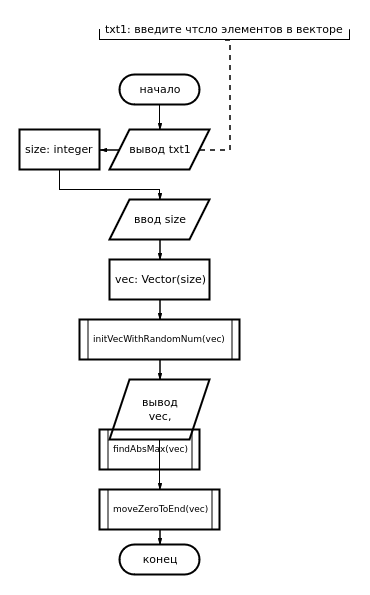
\includegraphics[width=0.8\textwidth]{data/diagram18_1.png}
\end{figure}
% \newpage
\subsection{Код:}
\verbatiminput{data/task18_1.cpp}
\href{https://raw.githubusercontent.com/John1400800/stuff/refs/heads/main/c_learning/home_works/task18_1.cpp}{source
code}
\subsection{Результат работы программы:}
\begin{figure}[H]
  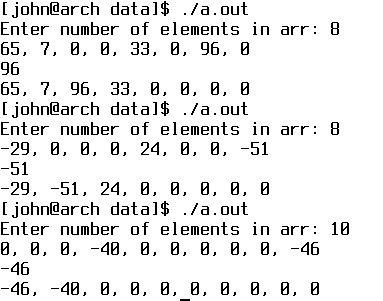
\includegraphics[width=0.8\textwidth]{data/demo18_1.png}
\end{figure}
\section*{Задание 2}
\setcounter{subsection}{0}
\subsection{Условие:}
\begin{enumerate}
  \item Разработать соответствующую варианту программу с использованием
    имеющегося описания, отладить ее и перерешать с использованием векторов.
  \item Подготовить набор тестов, подтверждающих правильность работы программы.
  \item Оформить отчет, включив в него постановку задачи коды программ и
    результаты их работы.
\end{enumerate}
\begin{quote}
  \begin{small}
    Задано описание:\\[1mm]

    \textsl{
      typedef float* Vector[100];\\
      Vector x;
    }

    Считая, что все элементы вектора x отличны от \textsl{NULL}, описать

    \begin{itemize}
      \item процедуру del(x), которая в векторе x все ссылки указывающие на
        повторяющиеся элементы заменяет значением NULL;
      \item процедуру Inp(x) – формирования вектора x;
      \item процедуру Out(x) – вывода чисел, на которые ссылаются элементы
        вектора x отличные от NULL.
    \end{itemize}
  \end{small}
\end{quote}
\subsection{Алгоритм / Мат. модель} 

\end{document}
